\documentclass{article}

% Language setting
% Replace `english' with e.g. `spanish' to change the document language
\usepackage[english]{babel}

% Set page size and margins
% Replace `letterpaper' with `a4paper' for UK/EU standard size

\usepackage[letterpaper,top=2cm,bottom=2cm,left=3cm,right=3cm,marginparwidth=1.75cm]{geometry}

% Useful packages
\usepackage{amsmath}
\usepackage{graphicx}
\usepackage[colorlinks=true, allcolors=blue]{hyperref}
\usepackage{authblk}

\title{\huge \textbf{Resurrected Cat Paradox : Challenging the Von Neumann-Wigner Interpretation of Quantum Mechanics}}

\author{Riddhiman Bhattacharya}

\date{July 5, 2023}

\begin{document}
\maketitle
\Large 
\begin{abstract}
\Large

The quantum measurement problem revolves around how the collapse of the wave function occurs. The Copenhagen Interpretation suggests that wave function collapse happens when a particle is measured. The Von Neumann-Wigner Interpretation, a sub-interpretation of the Copenhagen Interpretation, proposes that consciousness causes the collapse. While this idea is debated and mostly dismissed now, it raises paradoxical situations. Objects can have different states depending on measurement results, and these states can be changed without collapsing the wave function, leading to a modification of the observed past. The Resurrected Cat Paradox presents a novel challenge to the Von Neumann-Wigner Interpretation, utilizing the Delayed Choice Experiment and the concept of consciousness influencing collapse. Other objections to this interpretation have also been raised, such as the role of conscious life evolution.

\end{abstract}

\section{\Large Introduction}
\subsection{\Large Fundamentals of Quantum Mechanics}

\subsubsection{\Large Wavefunction}
In classical mechanics we can predict the position $x(t)$ and momentum $p(x,t)$ of a particle as a function of time(t) when given the initial conditions and the forces acting on the particle \cite{Griffiths2004Introduction}. However, in quantum mechanics that is not the case. Rather we attempt to find the wave function  $\psi(x,t)$ of the particle.

To calculate this wave function we need to solve the Schr\"{o}dinger equation:
\begin{equation}
i\hbar \frac{\partial \Psi}{\partial t} = -\frac{\hbar^2}{2m}
\frac{\partial^2 \Psi}{\partial x^2} + V \Psi
\label{eq:1}
\end{equation}

This seemingly arbitrary function has an important physical significance, given by Born's statistical interpretation: $\int_a^b |\Psi(x,t)|^2 dx$ signifies the probability of finding a particle between \textit{a} and \textit{b} at a time \textit{t} given its wave function


This means that quantum mechanics is indeterminate, that is, you cannot predict the outcome of any experiment, but you can gain statistical information about all the possible outcomes. However, we can say with certainty that the particle has to be somewhere in space and time. Therefore, we can normalise the wave function (provided it is square integrable).

\begin{equation}
\int\limits_{-\infty}^\infty |\Psi(x,t)|^2 dx = 1
\label{eq:2}
\end{equation}

This is useful for determining the magnitude of the complex multiplicative factor $A$ (note that we cannot determine the phase of $A$ by normalization), as if 

$\psi\left(\mathbit{x},\mathbit{t}\right)$ is a solution to (1), so is 
$A\cdot{\psi}\left(\mathbit{x},\mathbit{t}\right)$. 


%\begin{multline*}
 % \small \displaystyle f:[a,b]\to \mathbb %{C} {\text{ square integrable on %}}[a,b]\quad \iff \quad\\
  %\int _{a}^{b}|f(x)|^{2}\,\mathrm {d} %x<\infty 
%\label{eq:4}  
%\end{multline*}


\begin{align}
f:[a,b] &\to \mathbb{C} \text{ square integrable on } [a,b] \\
\iff \quad &\int_{a}^{b} |f(x)|^{2} \, dx < \infty
\end{align}


An important consequence of the Schrödinger equation is that if a wave function is normalized at any time, the normalization remains preserved  \cite{Griffiths2004Introduction}.  If the normalization hadn't been preserved, then all wave functions would become non-normalizable (not physical states) and the whole theory would collapse as the Born's interpretation would be deemed incompatible with the Schr\"{o}dinger's equation.


\subsubsection{\Large What happens when you make a measurement?}

Let us assume an arbitrary wave function of a particle \ref{fig:Before measurement}, with probabilities of being at different points.


%ADD MORE

\begin{figure}
\centering
     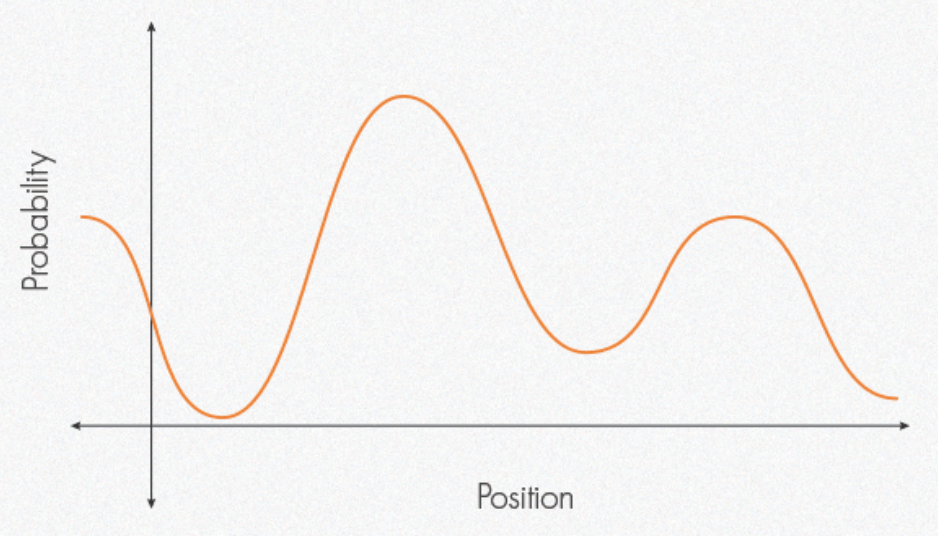
\includegraphics[width=7.5cm,height=7.5cm,keepaspectratio]{Wavefunction before measurement.png}
      \caption{An arbitrary wave function with different probabilities of finding the particle at different points}
       \label{fig:Before measurement}
\end{figure}



The figure in \ref{fig:collapse} represents the Dirac delta function
\begin{equation}
    \delta (x)={\begin{cases}+\infty ,&x=0\\0,&x\neq 0\end{cases}}
    \label{eq:4}\\
    \ \text{Where:} \int _{-\infty }^{\infty }\delta (x)\,dx=1.
\end{equation}

\begin{figure}
\centering
     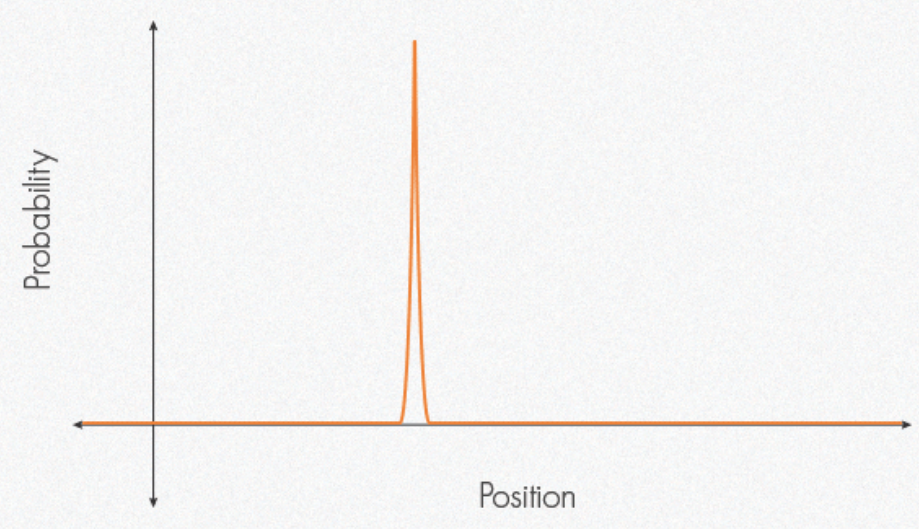
\includegraphics[width=7.5cm,height=7.5cm,keepaspectratio]{Wavefunction after collapse.png}
      \caption{The collapse of the wave function into a delta function when the particle was found at B }
       \label{fig:collapse}
\end{figure}




After the measurement, the wave function instantly spreads out, while obeying the Schr\"{o}dinger equation but with different initial conditions, so the wave function gets modified.

Now, the question arises, when we measured the particle to be at B at some time $t_0$ where is B \textbf{just before} the measurement?

There are three different positions scientists take on this question:
\begin{itemize}
\item \textbf{The realist position}: The realist believes that the particle was at C and quantum mechanics could not predict it, making it an ”incomplete theory” that needs a hidden variable along with the wave function for it to be rendered complete. They believed that nothing is indeterminate and that indeterminacy is just a reflection of our ignorance. 
\item \textbf{The orthodox position}: The particle was not anywhere. You only know where the particle is when you make a measurement, otherwise, its position is indeterminate, and it can be anywhere. We compel the particle to attain a definite position by measuring it. 
\item The agnostic position: The agonist believes that the in-determinacy problem is indeterminable. Because you must make a measurement to know the state of a system, you cannot know the state of a system between measurements. 
\end{itemize}
Interestingly Albert Einstein was a realist, as he believed quantum mechanics defied causality.

All these positions were popular among scientists until Bell's theorem was postulated.


This "\textbf{indeterminacy}" of Quantum mechanics leads to a fundamental quantum mechanical principle.


\subsection{\Large Von Neumann–Wigner Interpretation}

The \textbf{Von Neumann-Wigner Interpretation} is a variant of the \textbf{Copenhagen Interpretation} was developed by \textbf{John von Neumann} and \textbf{Eugene Wigner} and proposes a unique perspective on the collapse of the wave function.

According to the Von Neumann-Wigner Interpretation, \textbf{wave function collapse occurs when a conscious observer interacts with a quantum system.} In this view, the act of measurement is not just a physical process but is also intimately tied to consciousness. The collapse of the wave function happens as a result of the interaction between the measured system and the mind of the observer.

In this interpretation, the role of consciousness is central to the collapse process. It suggests that the observer's consciousness is responsible for determining the outcome of a measurement. The collapse is not seen as an objective, external event but rather as a subjective experience tied to the observer's consciousness.

The Von Neumann-Wigner Interpretation also introduces the idea of the \textbf{mind being the only measurement apparatus}. According to this view, the mind plays a unique role in the collapse of the wave function and is distinct from any physical measurement apparatus used in experiments.

.

\section{\Large Double Slit Experiment}
Thomas Young first conducted the Double-Slit Experiment in 1801 to display the wave-like behavior of light. In
the experiment, light is sent through two slits into a screen,
and an interference pattern emerges, which is the expected
result for objects displaying wave-like behavior. Later, other
variations of the experiment were conducted with beams of
electrons instead of light.

\begin{figure}[h]
\centering
     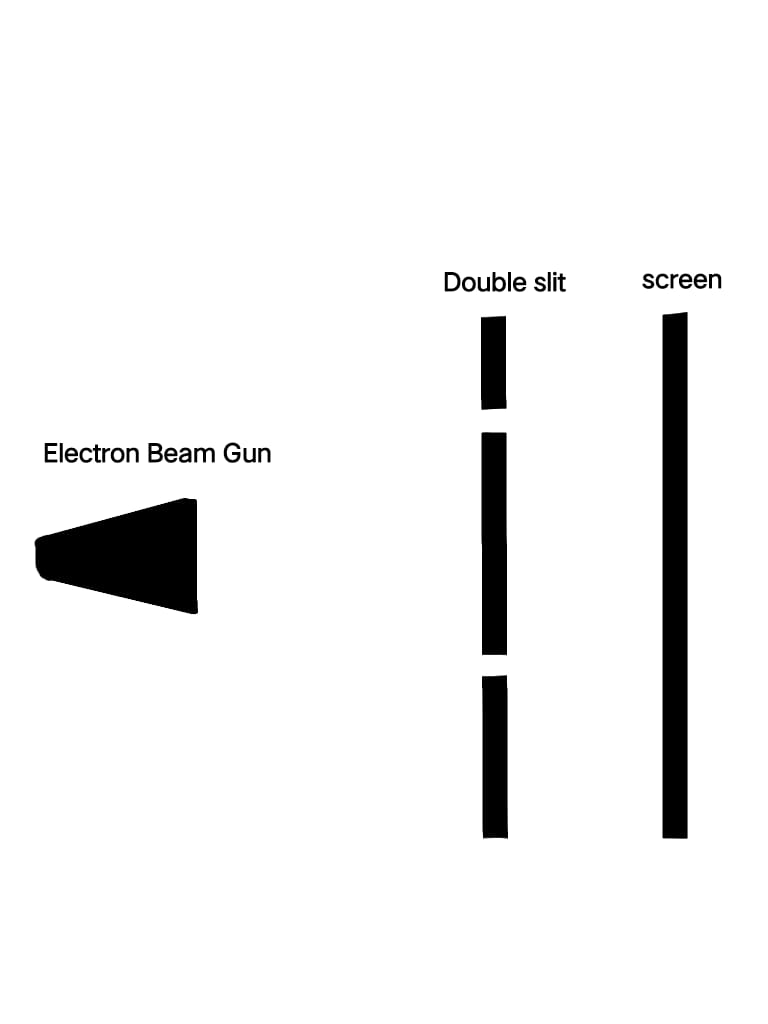
\includegraphics[width=7.5cm,height=7.5cm,keepaspectratio]{Double Slit.jpeg}
      \caption{Double Slit Experiment}
       \label{fig:DSE}
\end{figure}

In the modern Double-Slit Experiment, electrons are shot
to a screen through two slits. These electrons are expected
to behave like particles and create a clumped pattern on the
net. However, these electrons generate an interference pattern displaying wave-like behavior. Physicists thought that
these electrons must be interfering with each other. Despite
that, when the electrons are shot one by one, the interference
pattern is created again, showing that the electrons are interfering with themselves and not with other electrons. The
electrons pass through both slits simultaneously and show
wave-like behavior when shot. The electrons are not particles
or waves before measurement but rather wave functions. A
simple Double- Slit Experiment setup is given in Figure 1.
Since the electrons are in a superposition of two states, the
state of electrons that have been shot can be represented


\begin{equation}
    |\Psi\rangle=\frac{1}{\sqrt{2}}|right slit\rangle+ \frac{1}{\sqrt{2}}|left slit\rangle
\end{equation}



\subsection{\Large Observer Effects in Double Slit Experiment}

When a measuring device is put before the slits identifying which slit each electron is passing through (gathering the
“which-path” information), the interference pattern disappears, and a clumped pattern emerges. This means that the
electrons display particle-like behavior when a measurement
device is present. The act of measurement changes the outcome of the experiment.
When the measurement is made, the wave function collapses, and the electrons behave as particles. In fact, the wave
function collapses if the “which-path” information is known.
This is a key point for the following sections. A setup for
the Double-Slit Experiment with observer effects is given in
Figure 2.

Since measurement has been made and the wave functions
of the electrons have collapsed, the state of electrons can be
represented as:

\begin{equation}
    |\Psi\rangle=\frac{1}{1}|right slit\rangle+ \frac{0}{1}|left slit\rangle
\end{equation}

\begin{equation}
    |\Psi\rangle=\frac{0}{1}|right slit\rangle+ \frac{1}{1}|left slit\rangle
\end{equation}


\begin{figure}[h]
    \centering
    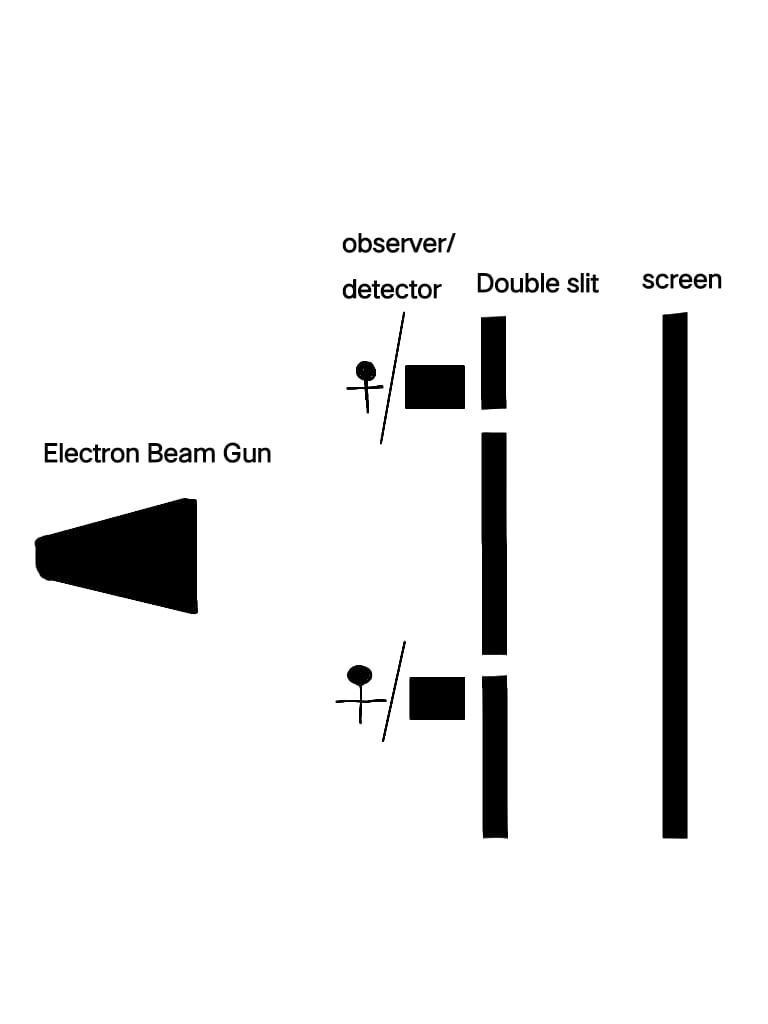
\includegraphics[width=5cm,height=7cm,keepaspectratio]{Observer Effects in Double Slit Experiment.jpeg}
    \caption{Caption}
    \label{Setup for Observer Effects }
\end{figure}




\section{\Large Delayed Choice experiment}

The Delayed Choice Experiment \ref{}, proposed by \textbf{John Wheeler}, is similar to the Double-Slit Experiment where the detectors are placed behind the slits, and measurements are made after the electrons pass through. 



\begin{figure}
    \centering [h]
    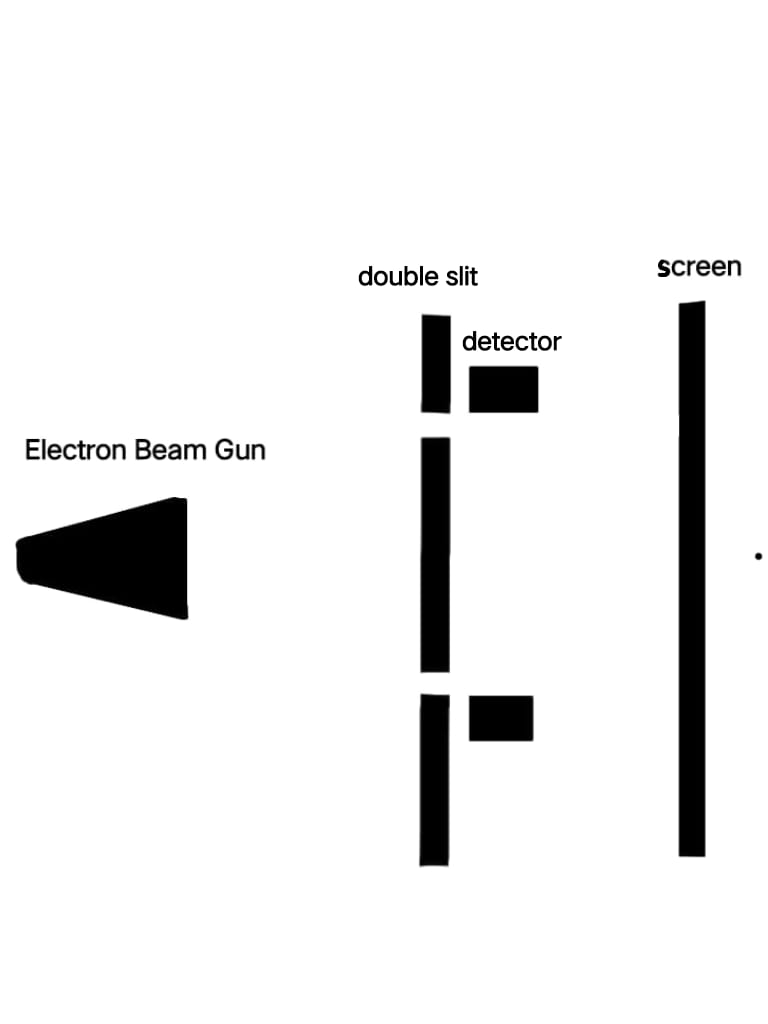
\includegraphics[width=10cm,height=7cm,keepaspectratio]{DCE.jpeg}
    \caption{Caption}
    \label{Setup for Delayed Choice Experiment}
\end{figure}

Surprisingly, even without measuring before the slits, a clumped pattern appears on the screen. This suggests that the electrons behave as wave functions, passing through both slits, but collapsing into a definite path after passing the slits. The experiment's outcome implies that the unobserved past can be altered.













\begin{figure}
\centering
     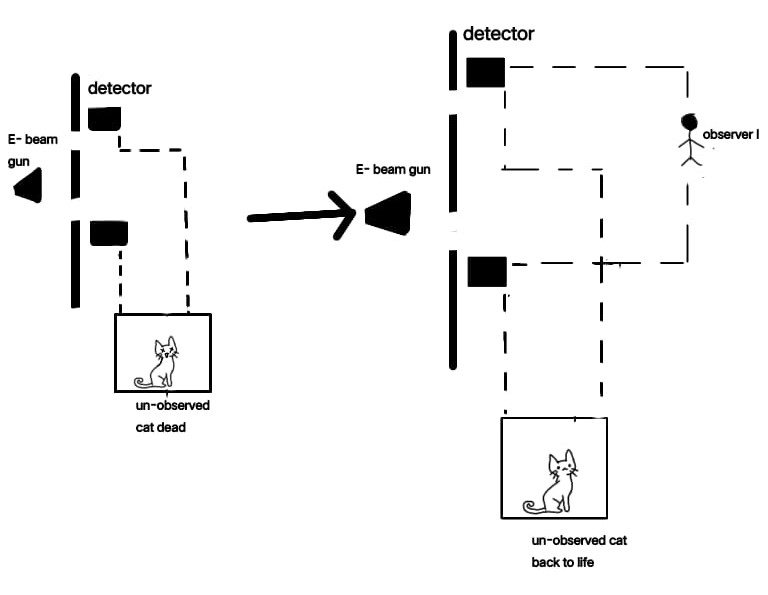
\includegraphics[width=10cm,height=7cm,keepaspectratio]{CASE-1,RCP.jpeg}
      \caption{Case-I}
       \label{}
\end{figure}

\Large 




\begin{figure}
\centering
     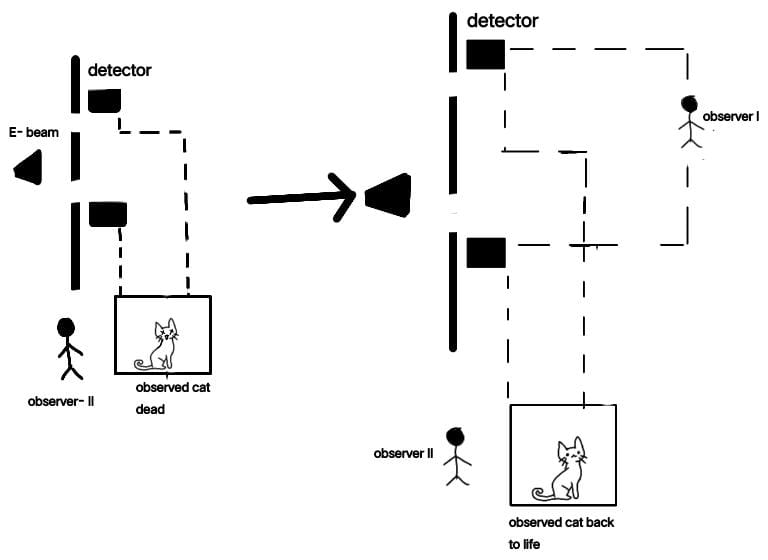
\includegraphics[width=10cm,height=7cm,keepaspectratio]{Case-2, RCP.jpeg}
      \caption{Case-II}
       \label{fig:Wavefn}
\end{figure}






















If the dead cat is taken out of the box after being observed
by observer II and later observer, I makes an observation, either we should end up with two cats, one dead and one alive,
which is against the fundamental laws of physics, or the observer
I's observation would not be able to change the past which
is against the premises of the experiment. Furthermore, the
more fundamental assumptions of the experiment, like the
observed past being altered and the cat returning to life after death, are not possible. Despite this, according to the Von
Neumann-Wigner Interpretation, the experiment itself is
not flawed. Thus, the Von Neumann-Wigner Interpretation
and the idea that consciousness causes wave function collapse
must be flawed.


\section{\Large The Resurrected Cat Paradox}


If we assume that the cat is not conscious, we can consider a thought experiment based on the Von Neumann-Wigner Interpretation. In this scenario:

1. When the electrons are shot without any observers making observations, the cat dies in a state where the particle goes through both slits simultaneously. According to the interpretation, the wave function is not collapsed without conscious awareness of the result.

2. After shooting the electrons and causing the cat's demise, if observer I makes an observation, something intriguing would occur. The interpretation suggests that the observation of observer I could potentially change the unobserved past, specifically the state of the electrons when they passed through the slits. This situation resembles the Delayed Choice Experiment.

3. If the past is altered due to observer I's observation, the cat's state would also change. In other words, it implies that the cat could come back to life as a consequence of the observation, even though it was initially dead.

This thought experiment highlights the peculiar consequences that could arise if the Von Neumann-Wigner Interpretation holds true and consciousness has a significant role in wave function collapse. It suggests that conscious observation could potentially influence not only the present but also the past, leading to changes in the state of physical objects like the cat.




\section{\Large Acknowledgment}
I extend my heartfelt gratitude to Ananya Mondal for her tremendous commitment and careful work in drawing all the diagrams used in the paper. The diagrams are an integral part of the paper that significantly improved the readability and comprehension of our work. She spent a lot of time refining them, and I'm very appreciative of that.



\bibliographystyle{alpha}
\bibliography{sample}

\end{document}
